\documentclass[12pt,a4paper]{article}

\usepackage{fontspec}
\usepackage{polyglossia}
\setdefaultlanguage{russian}
\setotherlanguage{english}
\IfFontExistsTF{Times New Roman}{%
  \setmainfont{Times New Roman}%
}{%
  \setmainfont{TeX Gyre Termes}%
}
\IfFontExistsTF{Courier New}{%
  \setmonofont{Courier New}%
  \newfontfamily\cyrillicfonttt{Courier New}%
}{%
  \setmonofont{CMU Typewriter Text}%
  \newfontfamily\cyrillicfonttt{CMU Typewriter Text}%
}

\usepackage{geometry}
\geometry{left=3cm,right=1.5cm,top=2cm,bottom=2cm}

\usepackage{graphicx}
\usepackage{float}
\usepackage{subcaption}
\usepackage{booktabs}
\usepackage{tabularx}
\usepackage{array}
\usepackage{enumitem}
\usepackage[hidelinks]{hyperref}

\setlength{\parindent}{1.25cm}
\setlength{\parskip}{0.35em}
\emergencystretch=2em
\hbadness=10000
\graphicspath{{./}}

\newcolumntype{Y}{>{\raggedright\arraybackslash}X}

\begin{document}

\begin{center}
    {\LARGE \textbf{Отчет}}
\end{center}

\section*{Ссылки и посылки}


GitHub: \href{https://github.com/karnaukhovGA69/SET9-69--}{https://github.com/karnaukhovGA69/SET9-69--}

\begin{table}[H]
    \centering
    \begin{tabularx}{\textwidth}{>{\centering\arraybackslash}p{1.6cm}Y}
        \toprule
        \textbf{Задача} & \textbf{Посылка} \\
        \midrule
        A1m & \href{https://dsahse25.contest.codeforces.com/group/SLdI1pWUpC/contest/691754/submission/375980010}{375980010} \\
        A1q & \href{https://dsahse25.contest.codeforces.com/group/SLdI1pWUpC/contest/691754/submission/375980021}{375980021} \\
        A1r & \href{https://dsahse25.contest.codeforces.com/group/SLdI1pWUpC/contest/691754/submission/375980403}{375980403} \\
        A1rq & \href{https://dsahse25.contest.codeforces.com/group/SLdI1pWUpC/contest/691754/submission/375980411}{375980411} \\
        \bottomrule
    \end{tabularx}
\end{table}

\section*{Графики}

\begin{figure}[H]
    \centering
    \begin{subfigure}[t]{0.49\textwidth}
        \centering
        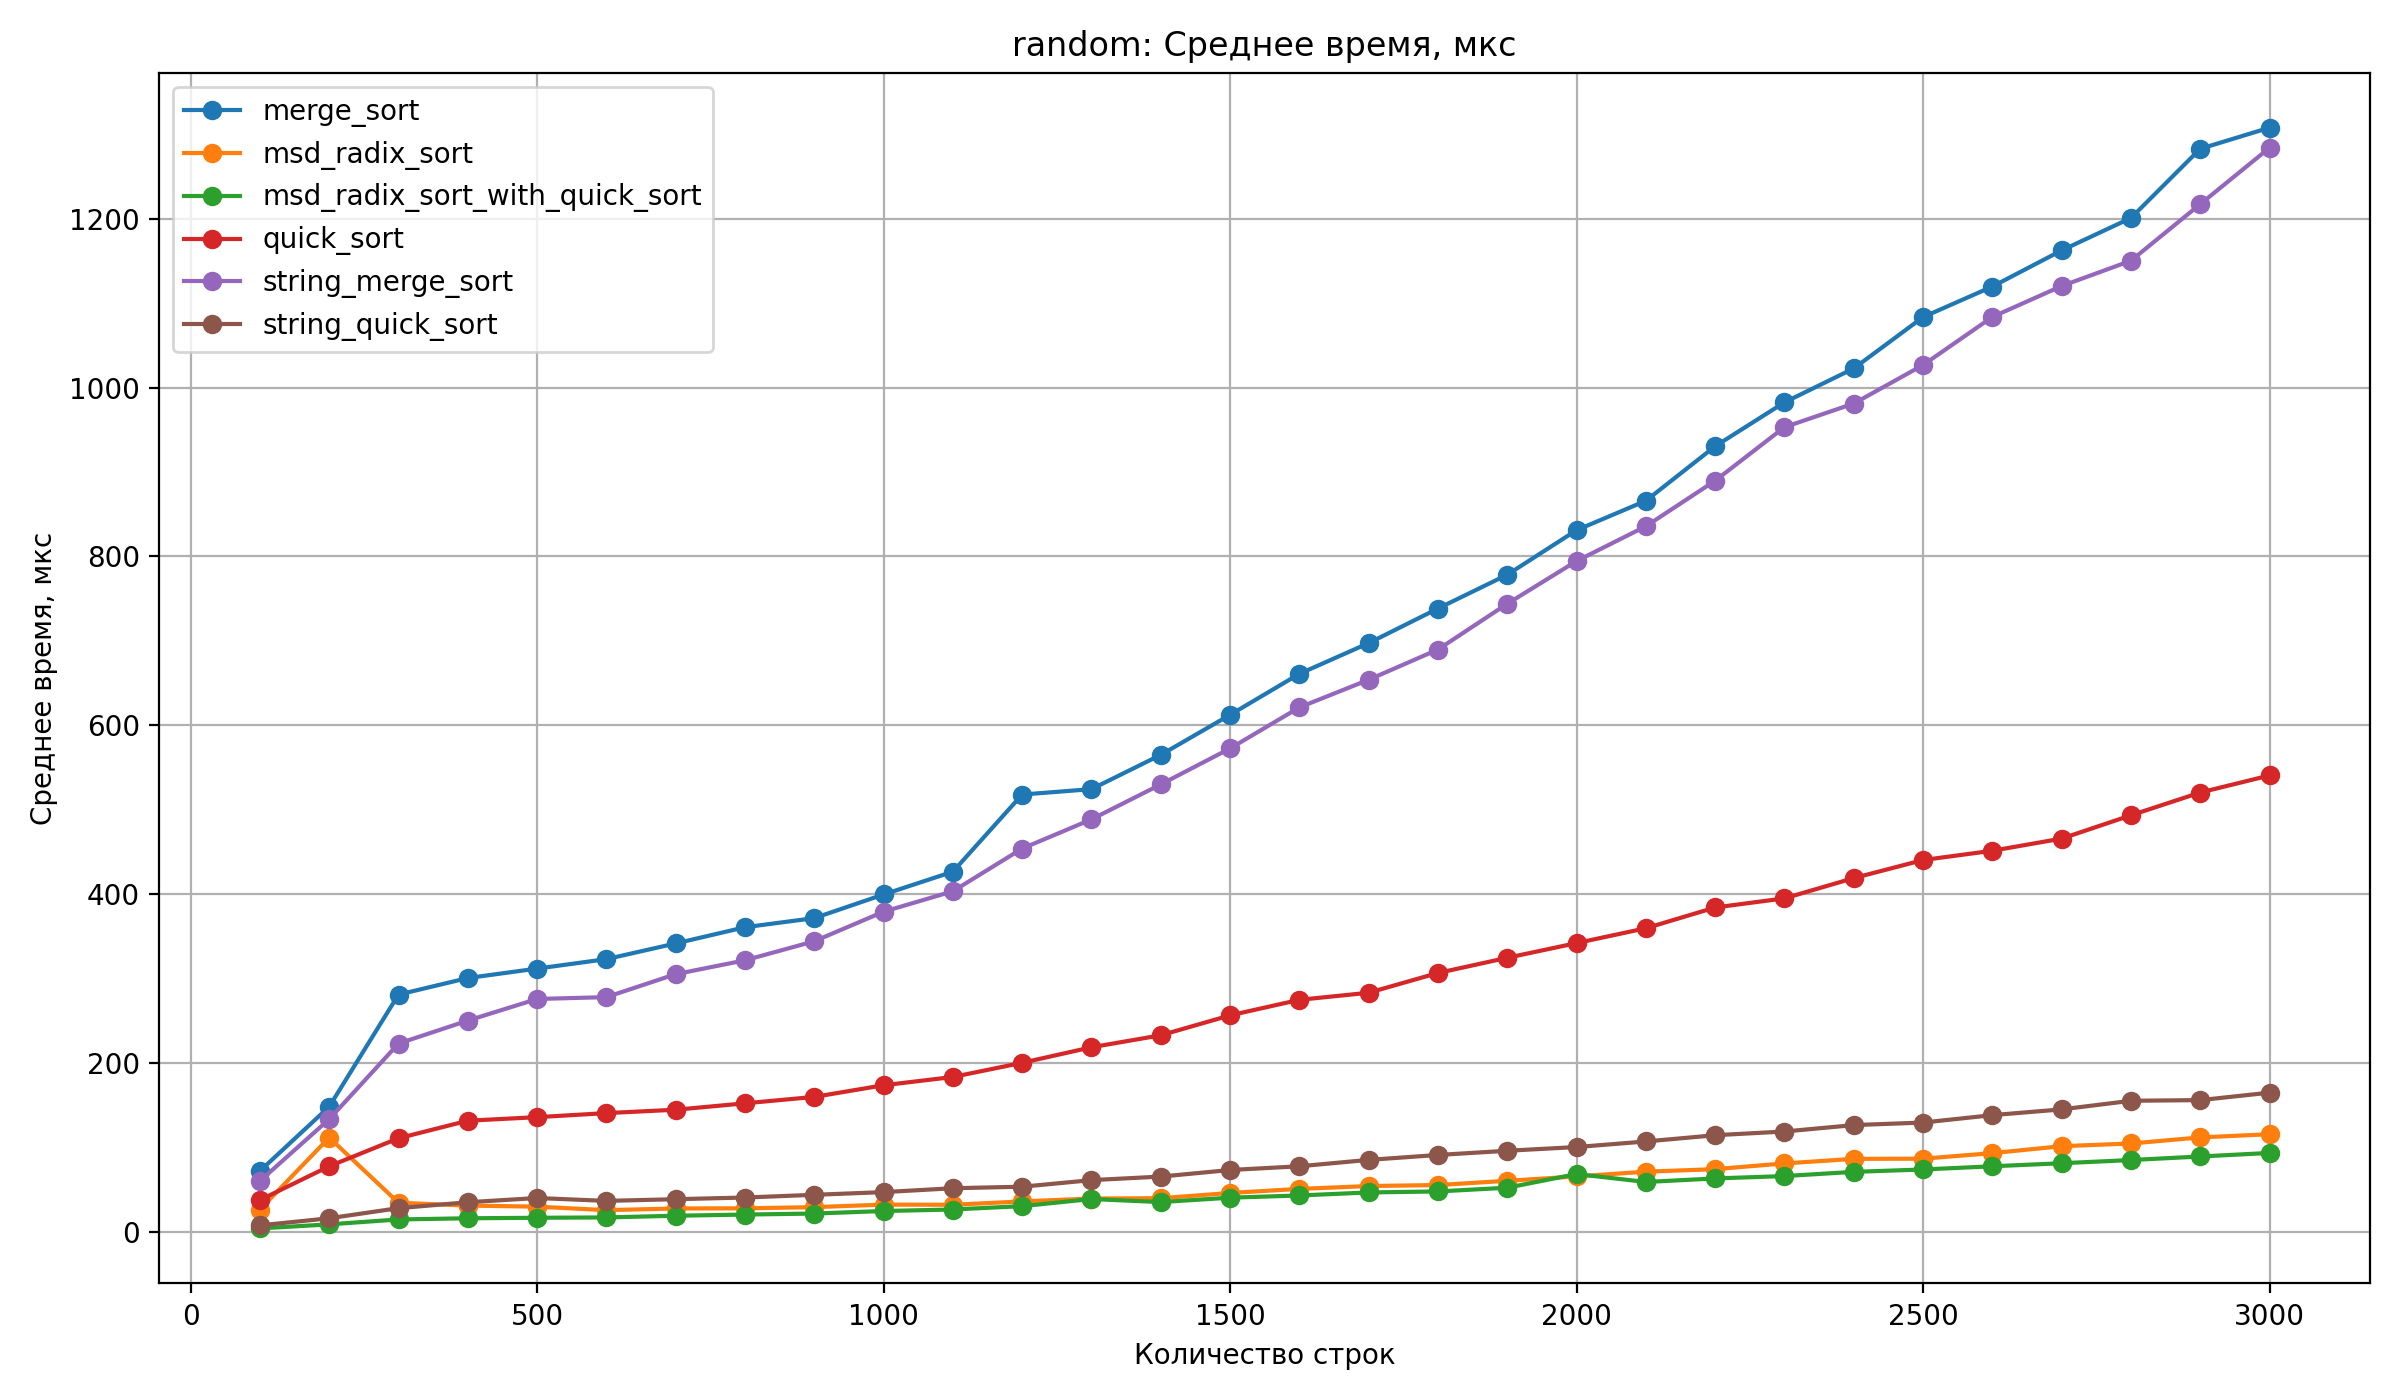
\includegraphics[width=\linewidth]{random_avg_time_us.png}
        \caption{Среднее время работы}
    \end{subfigure}
    \hfill
    \begin{subfigure}[t]{0.49\textwidth}
        \centering
        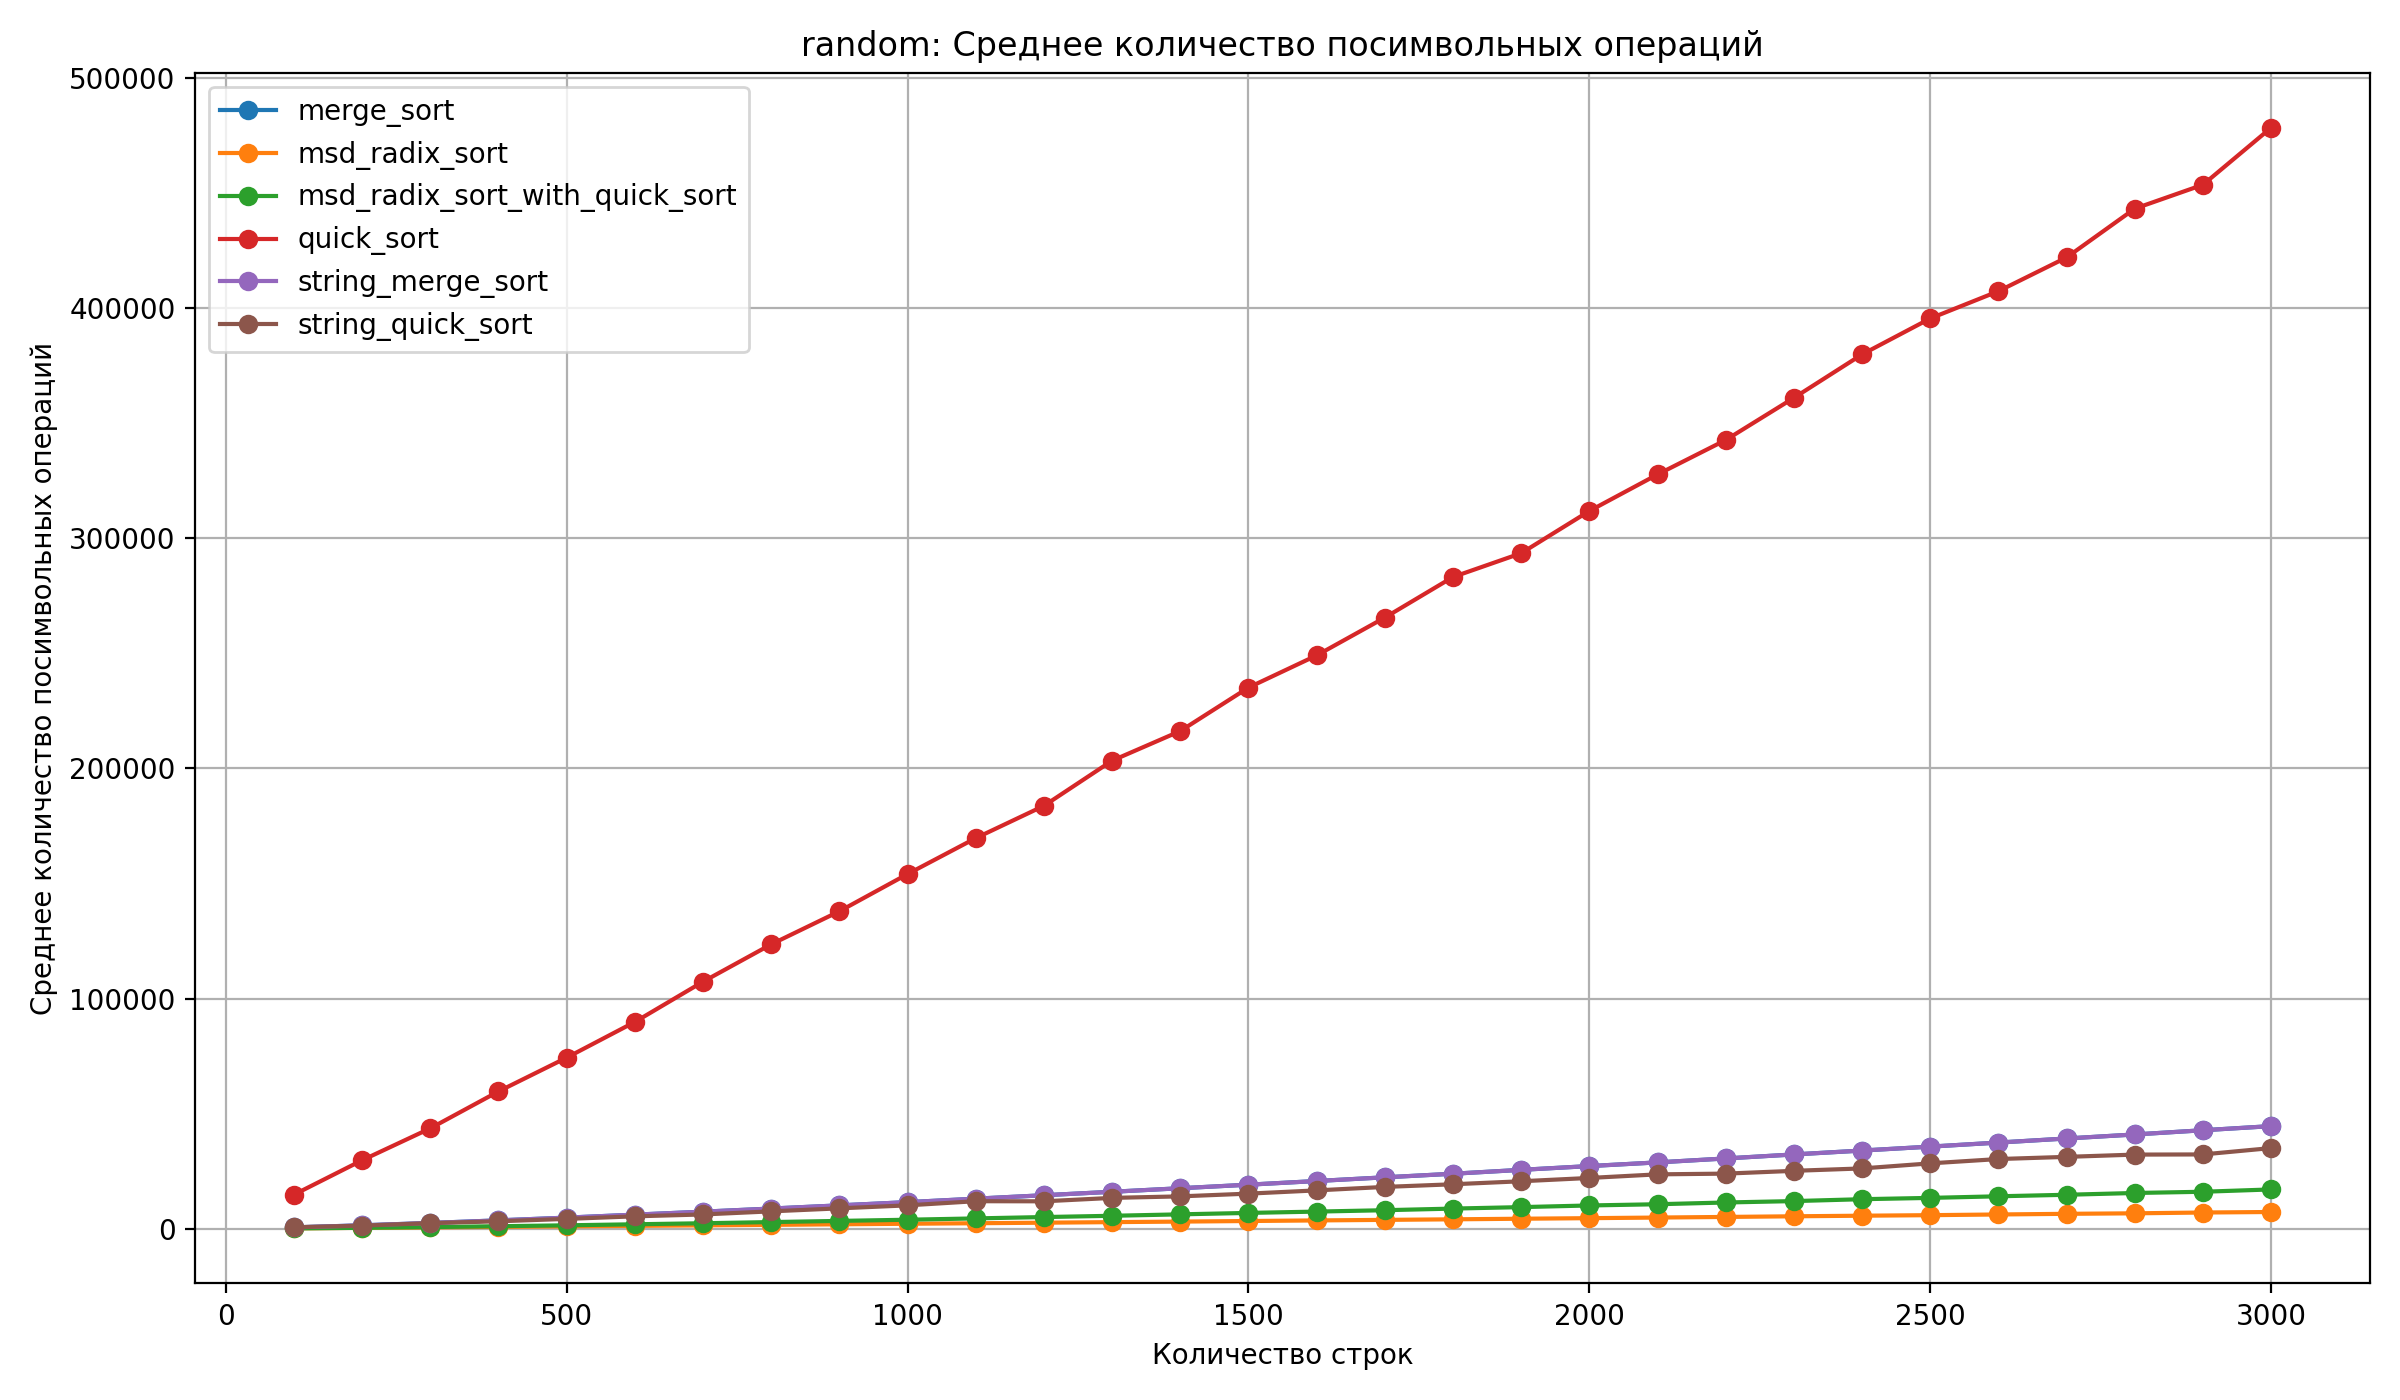
\includegraphics[width=\linewidth]{random_avg_symbol_operations.png}
        \caption{Среднее число посимвольных операций}
    \end{subfigure}
    \caption{Случайный набор строк}
\end{figure}

\begin{figure}[H]
    \centering
    \begin{subfigure}[t]{0.49\textwidth}
        \centering
        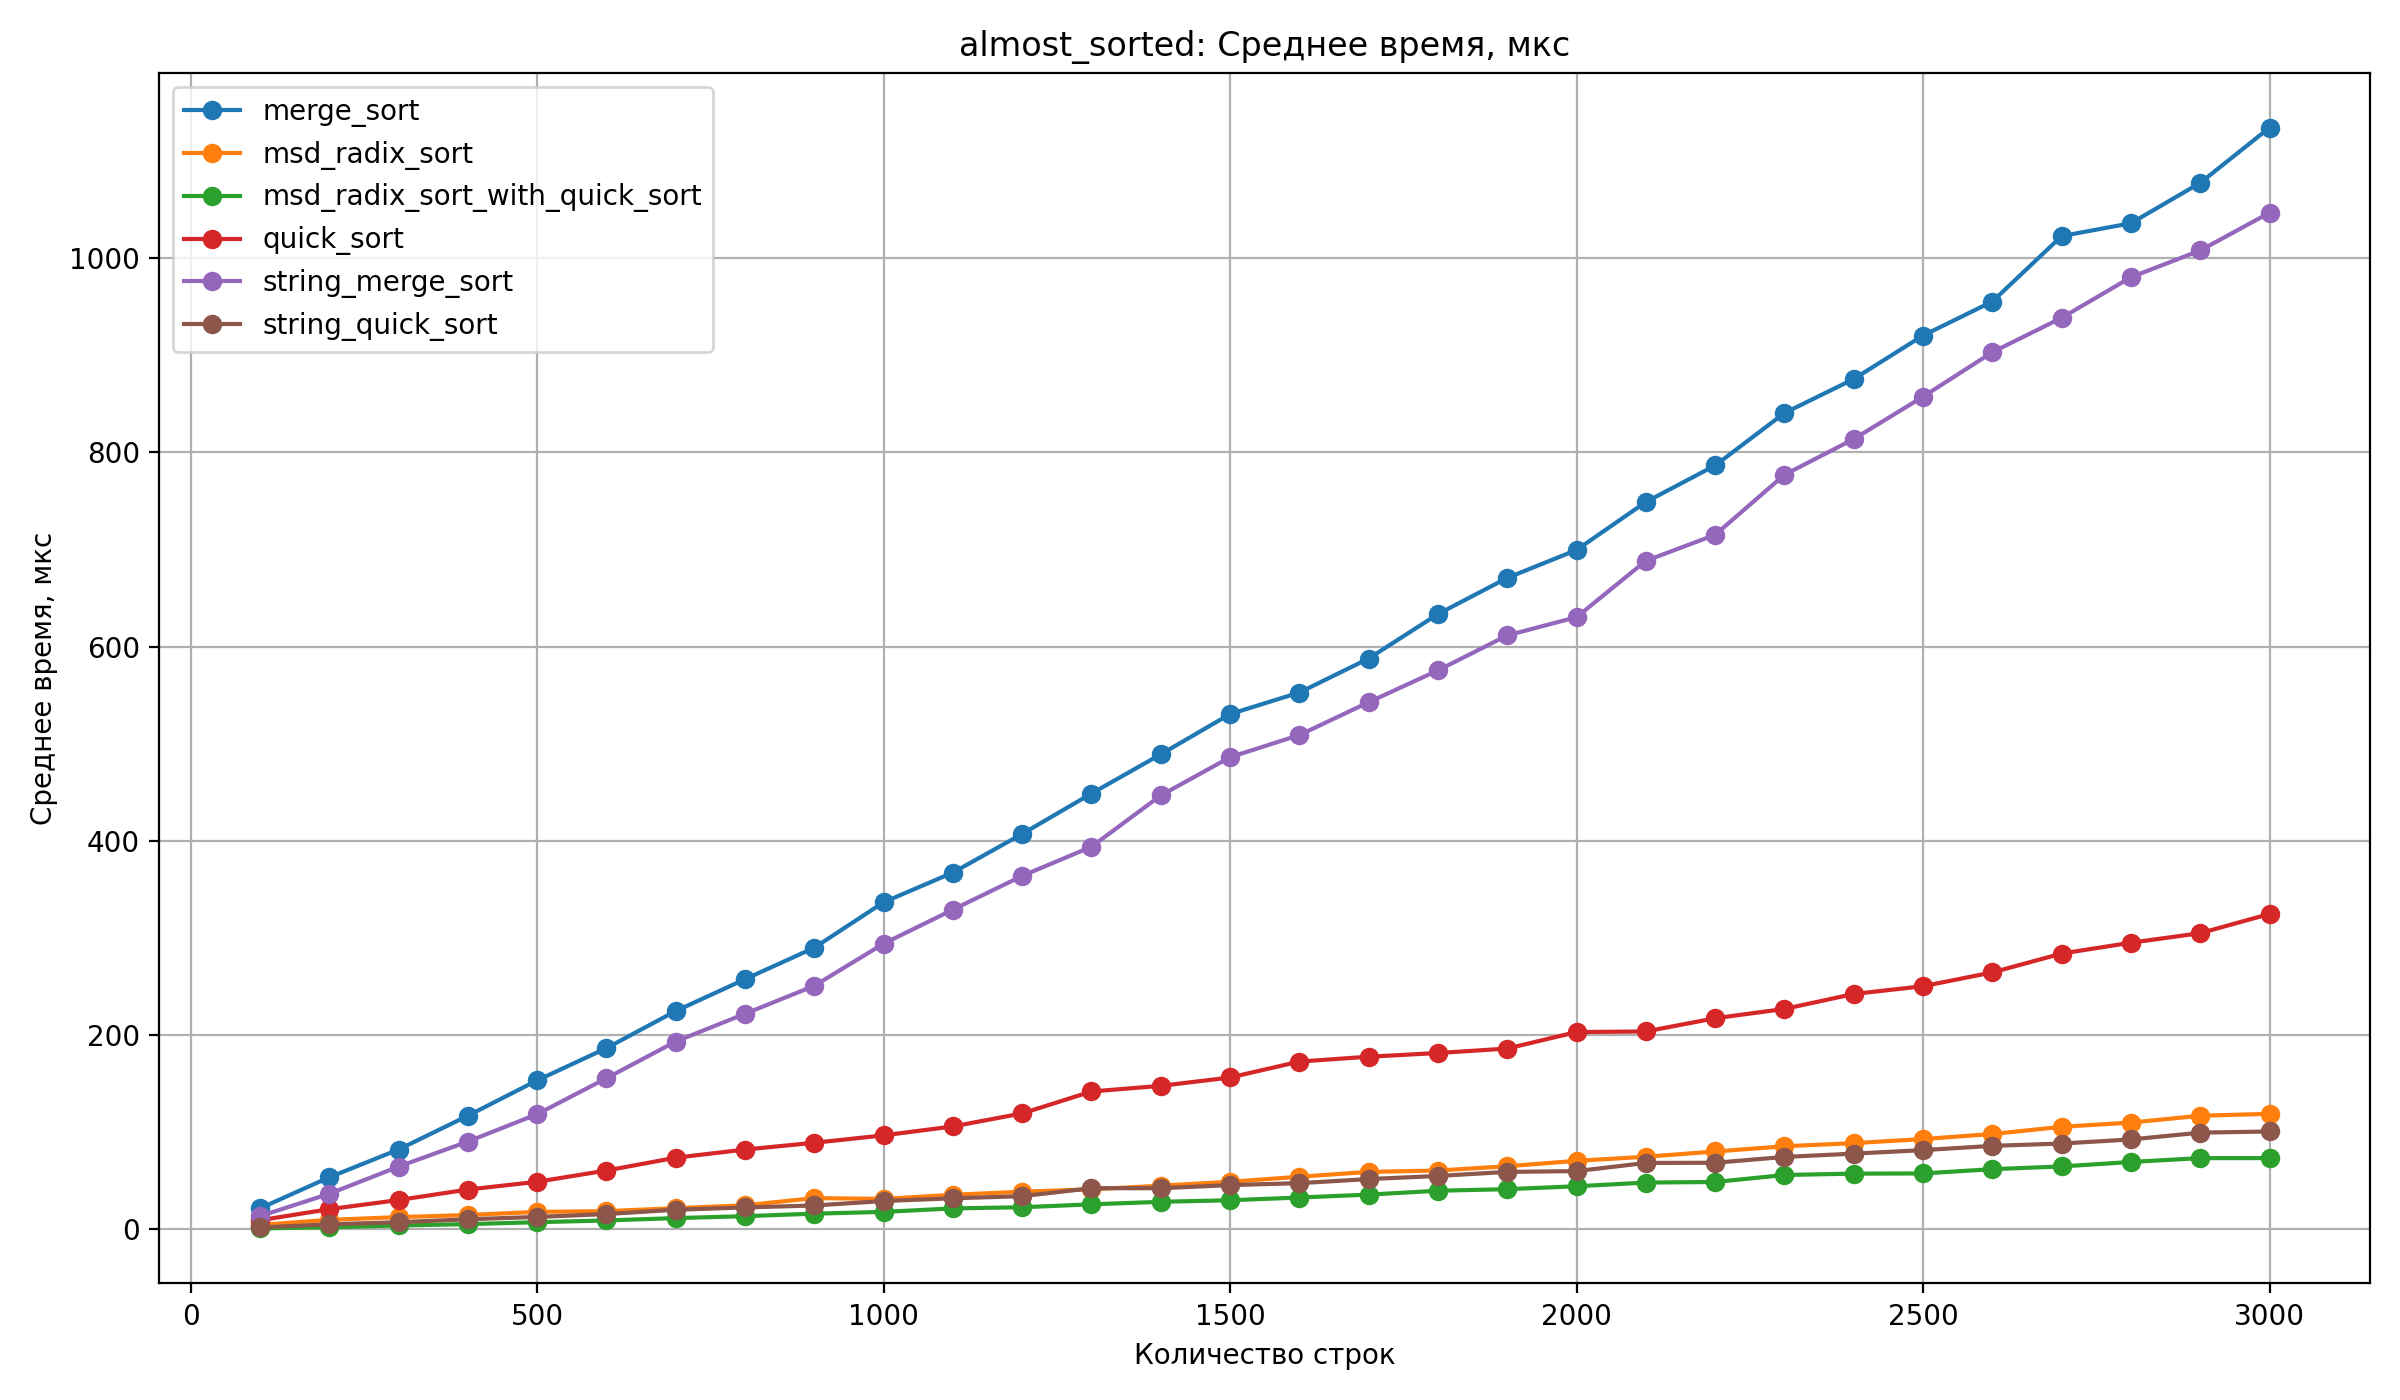
\includegraphics[width=\linewidth]{almost_sorted_avg_time_us.png}
        \caption{Среднее время работы}
    \end{subfigure}
    \hfill
    \begin{subfigure}[t]{0.49\textwidth}
        \centering
        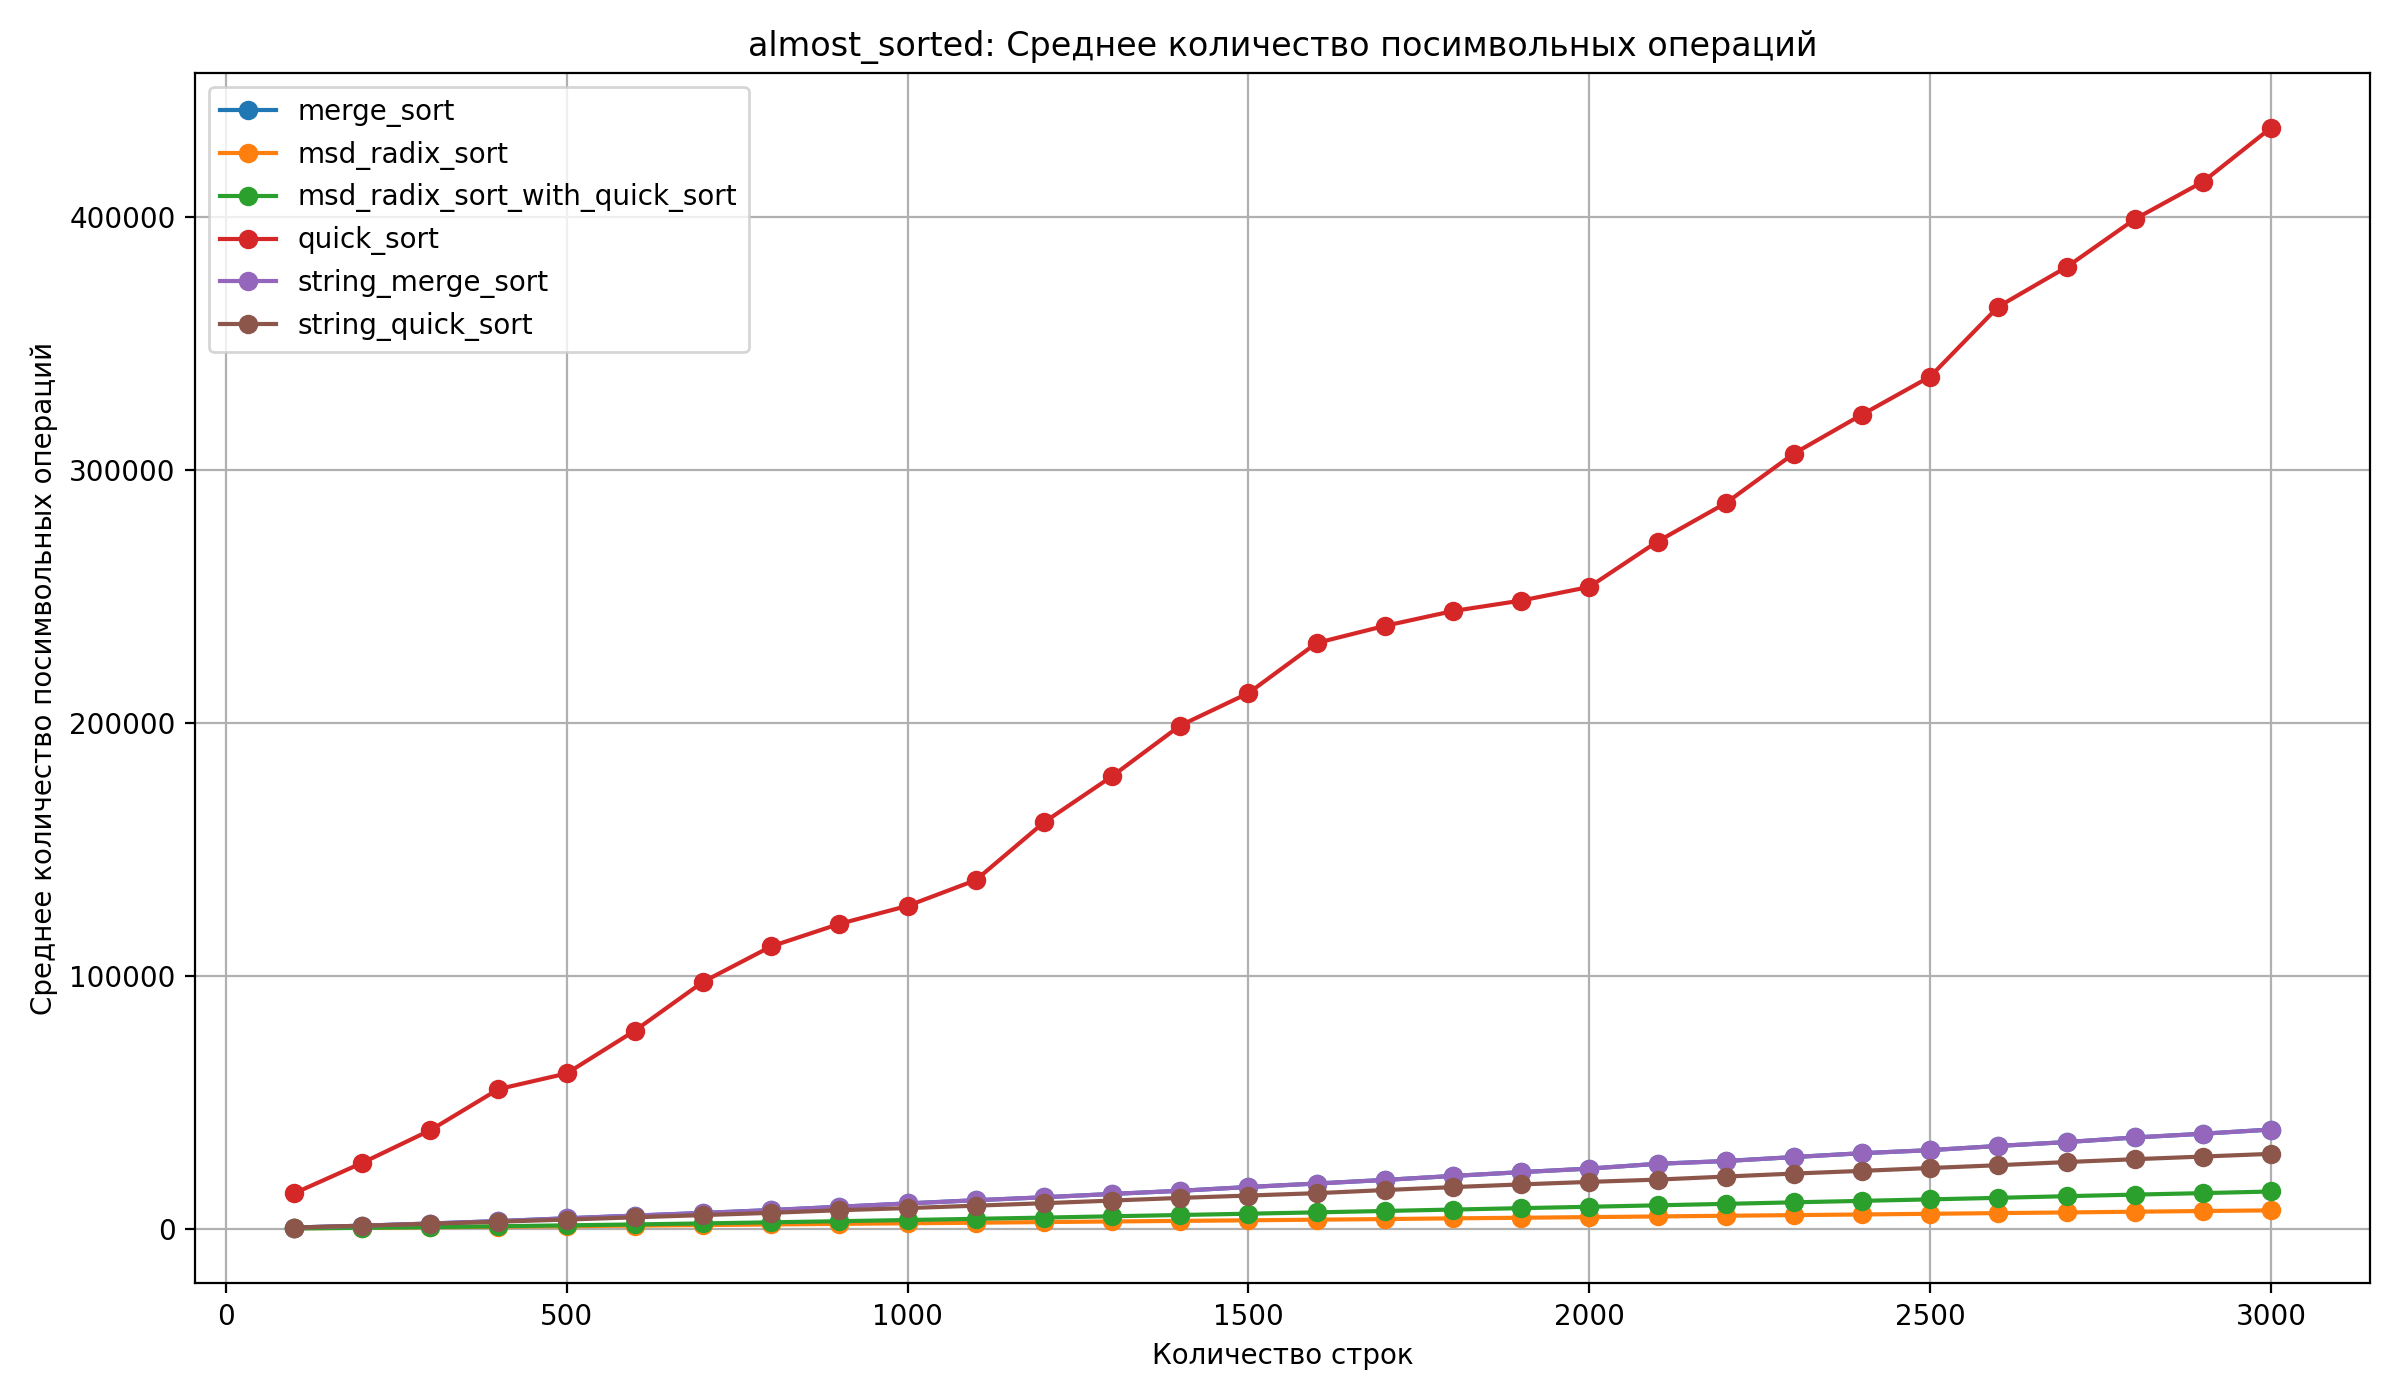
\includegraphics[width=\linewidth]{almost_sorted_avg_symbol_operations.png}
        \caption{Среднее число посимвольных операций}
    \end{subfigure}
    \caption{Почти отсортированный набор строк}
\end{figure}

\begin{figure}[H]
    \centering
    \begin{subfigure}[t]{0.49\textwidth}
        \centering
        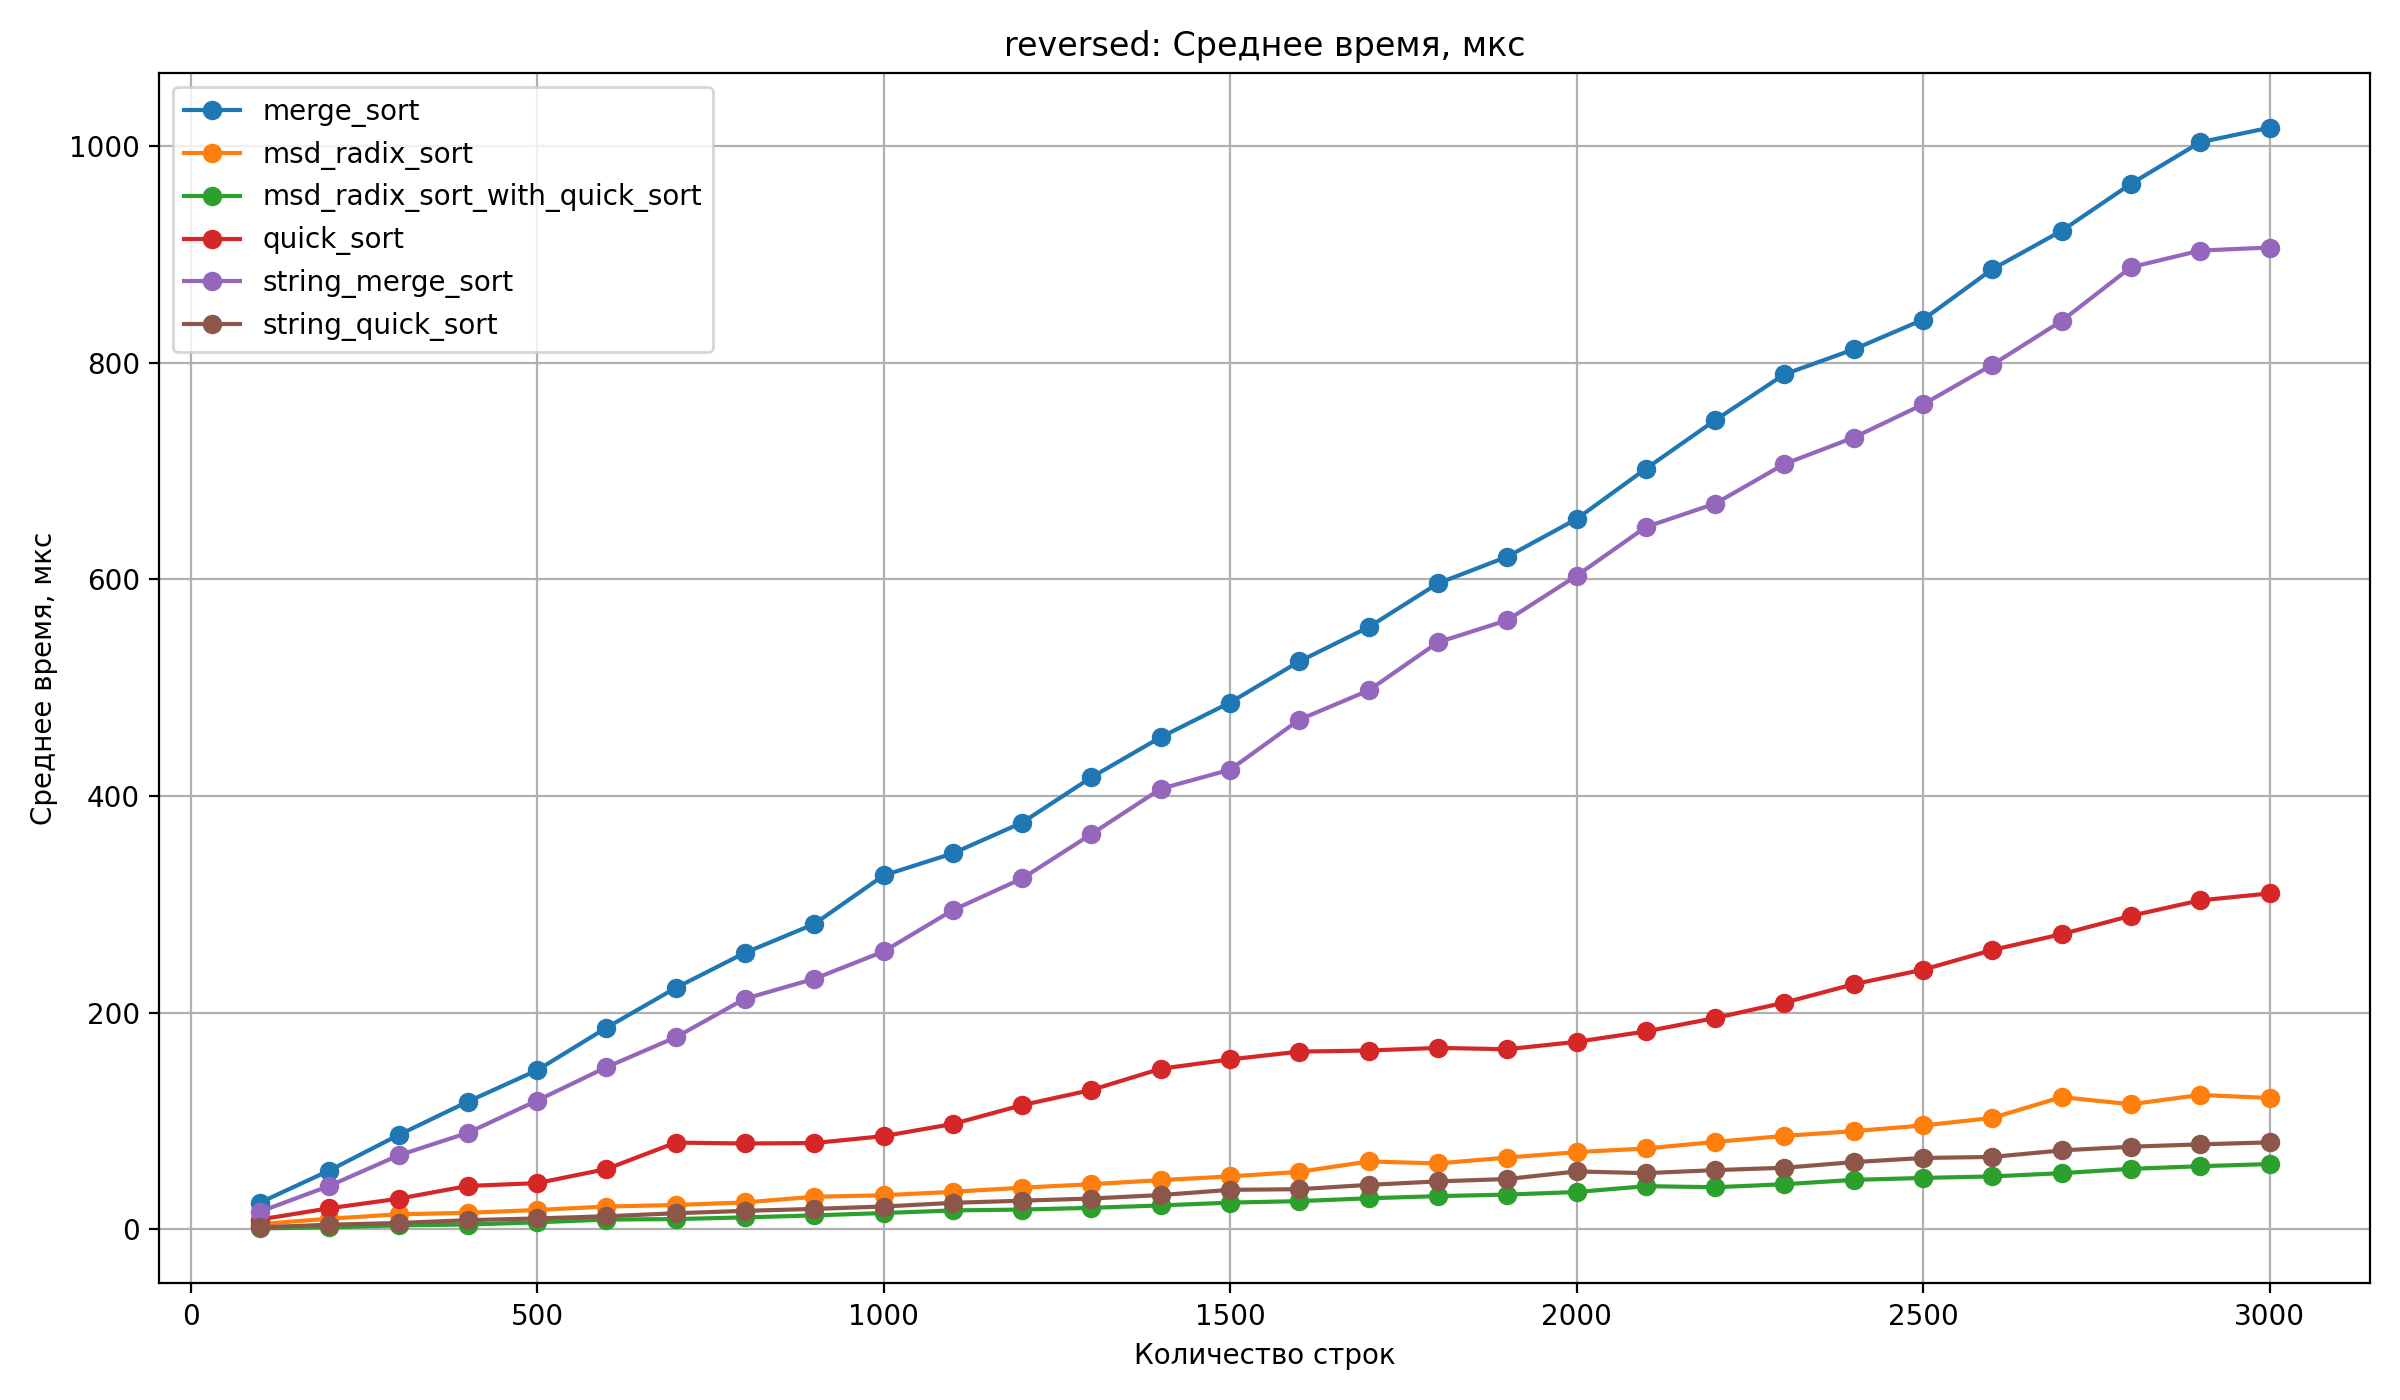
\includegraphics[width=\linewidth]{reversed_avg_time_us.png}
        \caption{Среднее время работы}
    \end{subfigure}
    \hfill
    \begin{subfigure}[t]{0.49\textwidth}
        \centering
        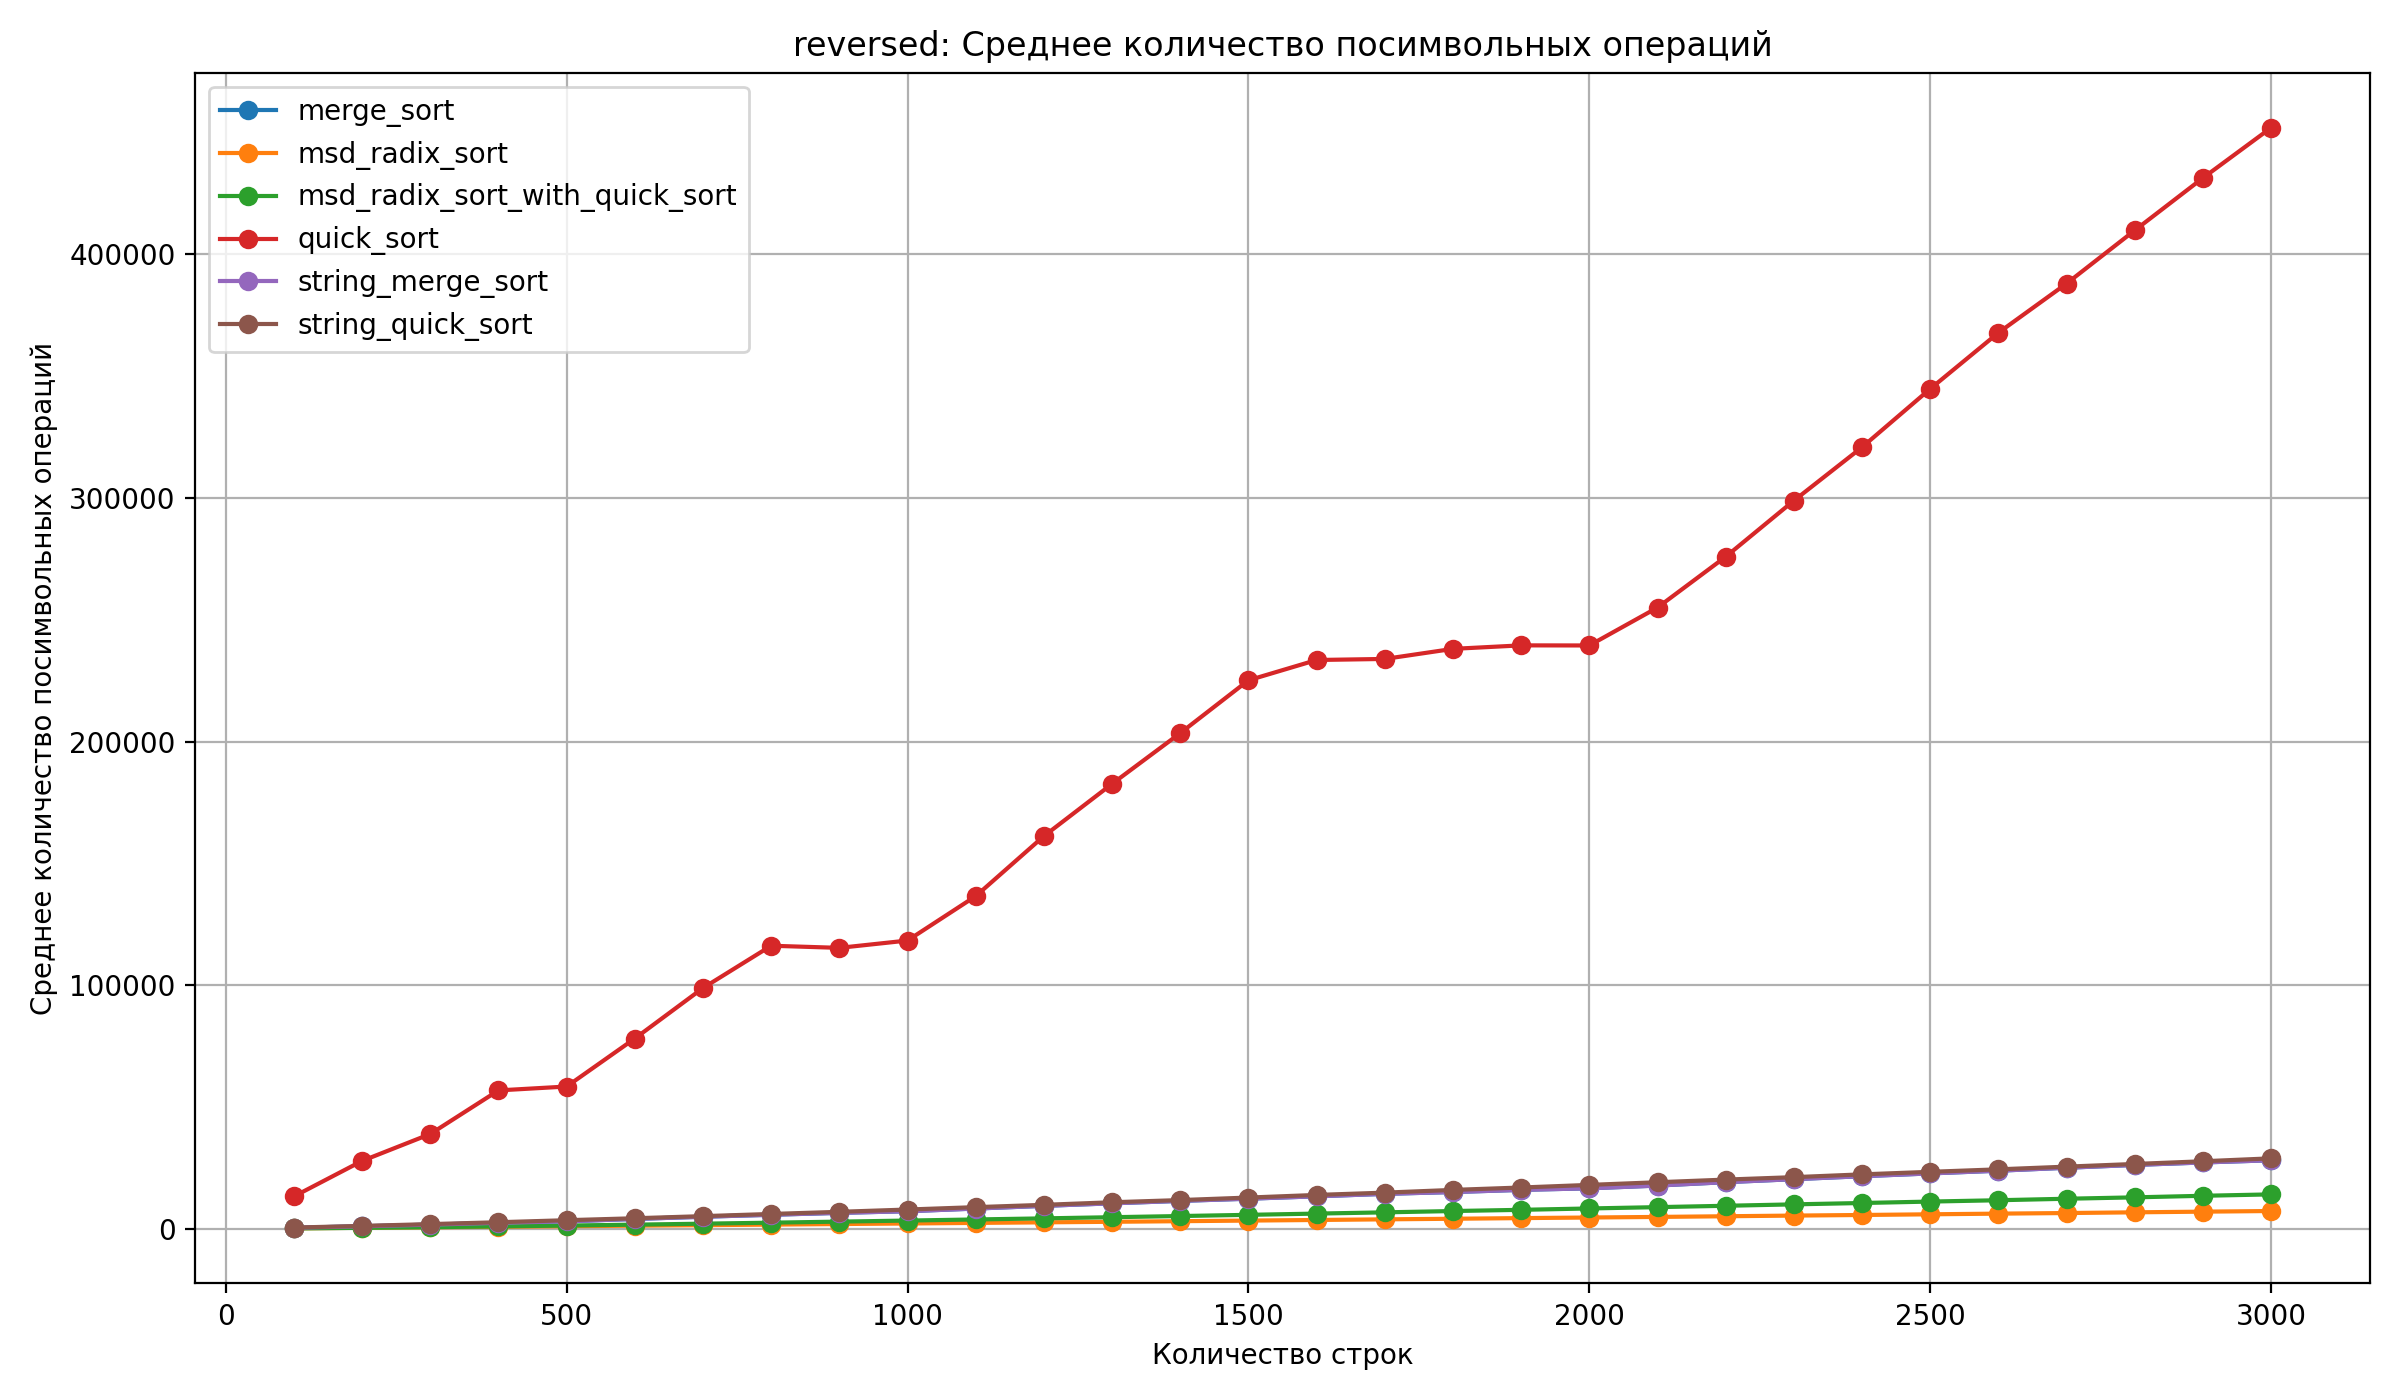
\includegraphics[width=\linewidth]{reversed_avg_symbol_operations.png}
        \caption{Среднее число посимвольных операций}
    \end{subfigure}
    \caption{Обратно отсортированный набор строк}
\end{figure}

\section*{Анализ результатов}

\begin{enumerate}[leftmargin=1.6em]
    \item \textbf{Время работы.}
    \begin{itemize}[leftmargin=1.4em]
        \item На наборах \texttt{random}, \texttt{almost\_sorted} и \texttt{reversed} самым быстрым оказался гибридный \texttt{MSD Radix Sort} с переходом на \texttt{QuickSort} для малых подмассивов. Он стабильно выигрывает по времени и заметно опережает остальные алгоритмы на больших входных данных.
        \item На тех же наборах обычный \texttt{MSD Radix Sort} чаще всего занимает второе или третье место. По времени он уступает гибридной версии, но все равно выглядит быстрее стандартных сравнительных сортировок.
        \item На строках с длинными общими префиксами лучший средний результат по времени показывает алгоритм \textit{Ternary String QuickSort}. 
        \item На больших входных данных стандартные \texttt{QuickSort} и \texttt{MergeSort} заметно уступают модифицированным строковым алгоритмам. Текущая реализация \textit{String MergeSort} по времени тоже не дает преимущества.
    \end{itemize}

    \item \textbf{Количество посимвольных операций.}
    \begin{itemize}[leftmargin=1.4em]
        \item На всех рассмотренных наборах минимальное число посимвольных проверок показывает обычный \texttt{MSD Radix Sort}. По данным эксперимента он остается лидером и на случайных строках, и на почти отсортированных, и на обратно отсортированных массивах.
        \item На тех же тестах гибридная версия работает быстрее, но из-за этого страдает число сравнений. При переключении на \texttt{QuickSort} на маленьких подмассивах она по операциям немного проигрывает чистому \texttt{MSD}.
        \item На всех наборах стандартный \texttt{QuickSort} дает самый высокий показатель посимвольных сравнений с большим отрывом. При полном сравнении строк его стоимость растет намного быстрее остальных алгоритмов.
        \item В текущих результатах \texttt{String MergeSort} не показывает преимущества относительно обычного \texttt{MergeSort}. Их кривые по числу операций почти совпадают, поэтому эффекта от оптимизации здесь не видно.
    \end{itemize}
\end{enumerate}

\end{document}
